%*******10********20********30********40********50********60********70********80

% For all chapters, use the newdefined chap{} instead of chapter{}
% This will make the text at the top-left of the page be the same as the chapter

\chap{Background Theory} % history of the jetpak

Lorem ipsum dolor sit amet, consectetur adipiscing elit. Vivamus at pulvinar nisi. Phasellus hendrerit, diam placerat interdum iaculis, mauris justo cursus risus, in viverra purus eros at ligula. Ut metus justo, consequat a tristique posuere, laoreet nec nibh. Etiam et scelerisque mauris. Phasellus vel massa magna. Ut non neque id tortor pharetra bibendum vitae sit amet nisi. Duis nec quam quam, sed euismod justo. Pellentesque eu tellus vitae ante tempus malesuada. Nunc accumsan, quam in congue consequat, lectus lectus dapibus erat, id aliquet urna neque at massa. Nulla facilisi. Morbi ullamcorper eleifend posuere. Donec libero leo, faucibus nec bibendum at, mattis et urna \cite{AWriter}. Proin consectetur, nunc ut imperdiet lobortis, magna neque tincidunt lectus, id iaculis nisi justo id nibh. Pellentesque vel sem in erat vulputate faucibus molestie ut lorem.

\begin{figure}
    \centering
    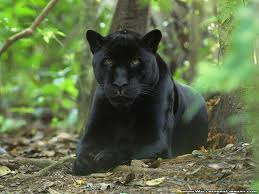
\includegraphics[scale=1, angle=0]{panther.jpg}
    \caption[The panther]{A panther is always watching}
    \label{fig: jordan}
\end{figure}

Duis nec quam quam, sed euismod justo. Pellentesque eu tellus vitae ante tempus malesuada. Nunc accumsan, quam in congue consequat, lectus lectus dapibus erat, id aliquet urna neque at massa. Nulla facilisi. Morbi ullamcorper eleifend posuere. Donec libero leo, faucibus nec bibendum at, mattis et urna. Proin consectetur, nunc ut imperdiet lobortis, magna neque tincidunt lectus, id iaculis nisi justo id nibh. Pellentesque vel sem in erat vulputate faucibus molestie ut lorem.


\begin{figure}
        \centering
        \begin{subfigure}[b]{0.4\textwidth}
                \centering        %   l   b   r   t
                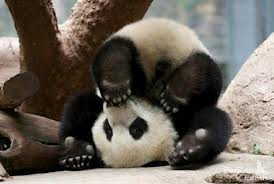
\includegraphics[trim=0.3cm 0cm 0cm 0cm, clip=true, 
                                width=\linewidth]
                                {panda.jpg}
                \caption{Panda}
                \label{subfig: ff}
        \end{subfigure}
        ~ % for a little horisontal distance
        \raisebox{3cm}[\height][\depth]{$\Rightarrow$}
        \hspace{0.2mm} % for a little horisontal distance
        \begin{subfigure}[b]{0.4\textwidth}
                \centering
                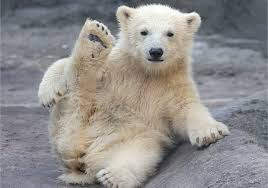
\includegraphics[trim=0cm 0cm 0cm 0cm, clip=true, 
                                width=\linewidth]
                                {polarbear.jpg}
                \caption{Polar bear}
                \label{subfig: sf}
        \end{subfigure}
        \caption[The panda-polar bear relationship ]
                {It is not widely known that the panda becomes a polar bear 
                when dressing up in the winter camouflage suite \cite{AnExpert}}
        \label{fig: pentagram}
\end{figure}




